\section{Background and Overview} \label{sec:background} \begin{figure*}[t]
\begin{center}
\begin{tabular}{ccc}
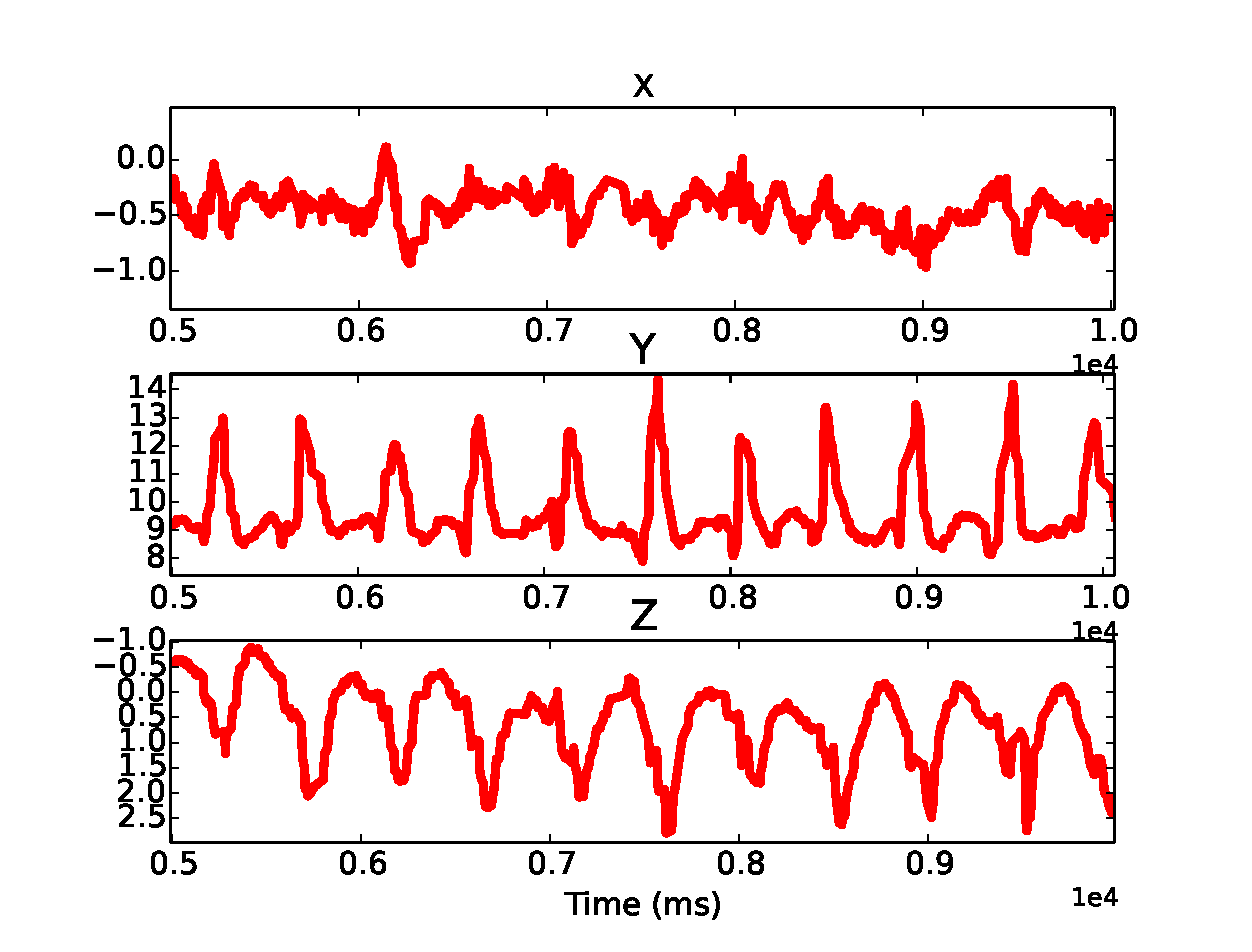
\includegraphics [width=.33\linewidth]{../mobisys_paper/fig/raw_sub1.eps}&
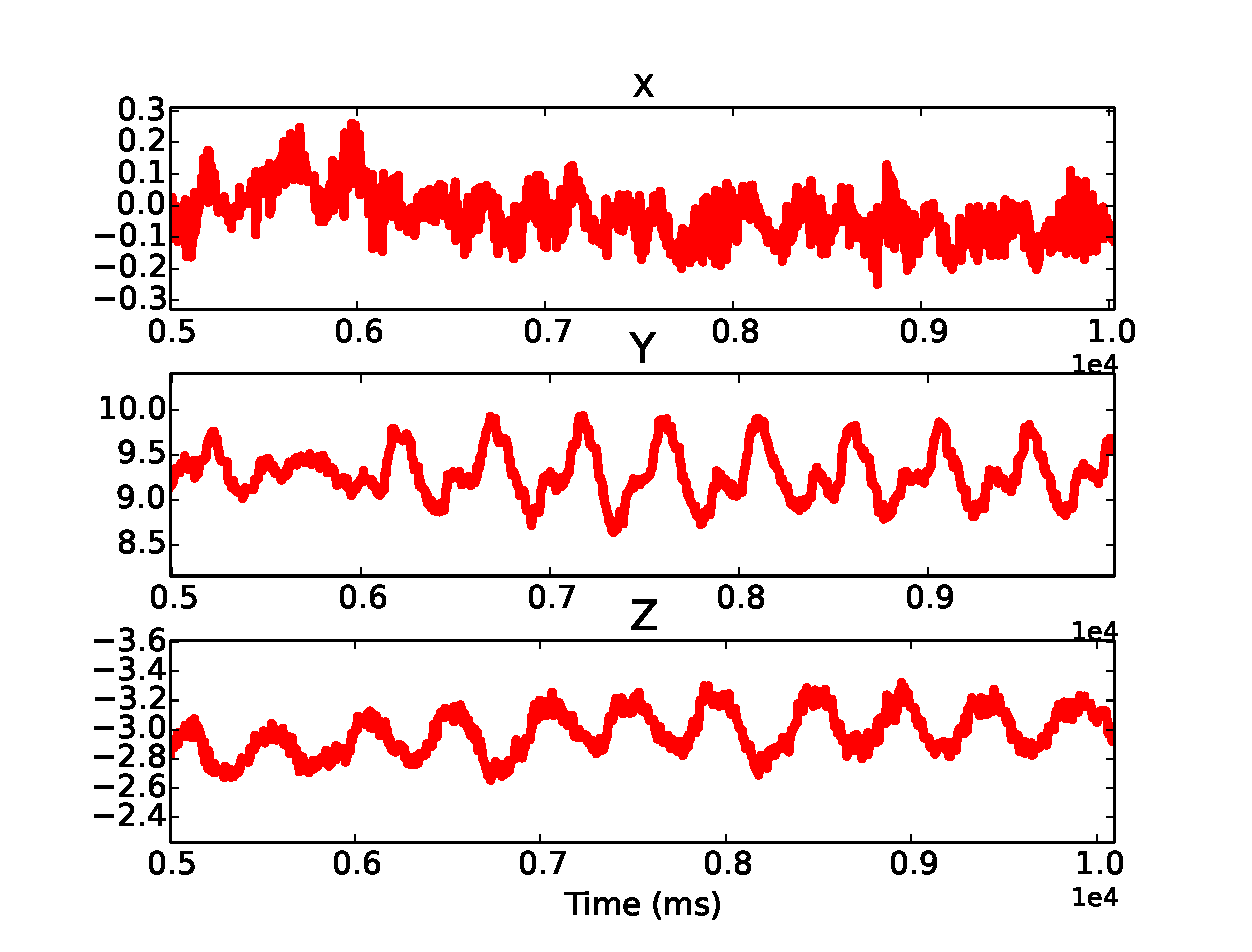
\includegraphics [width=.33\linewidth]{../mobisys_paper/fig/raw_sub8.eps}&
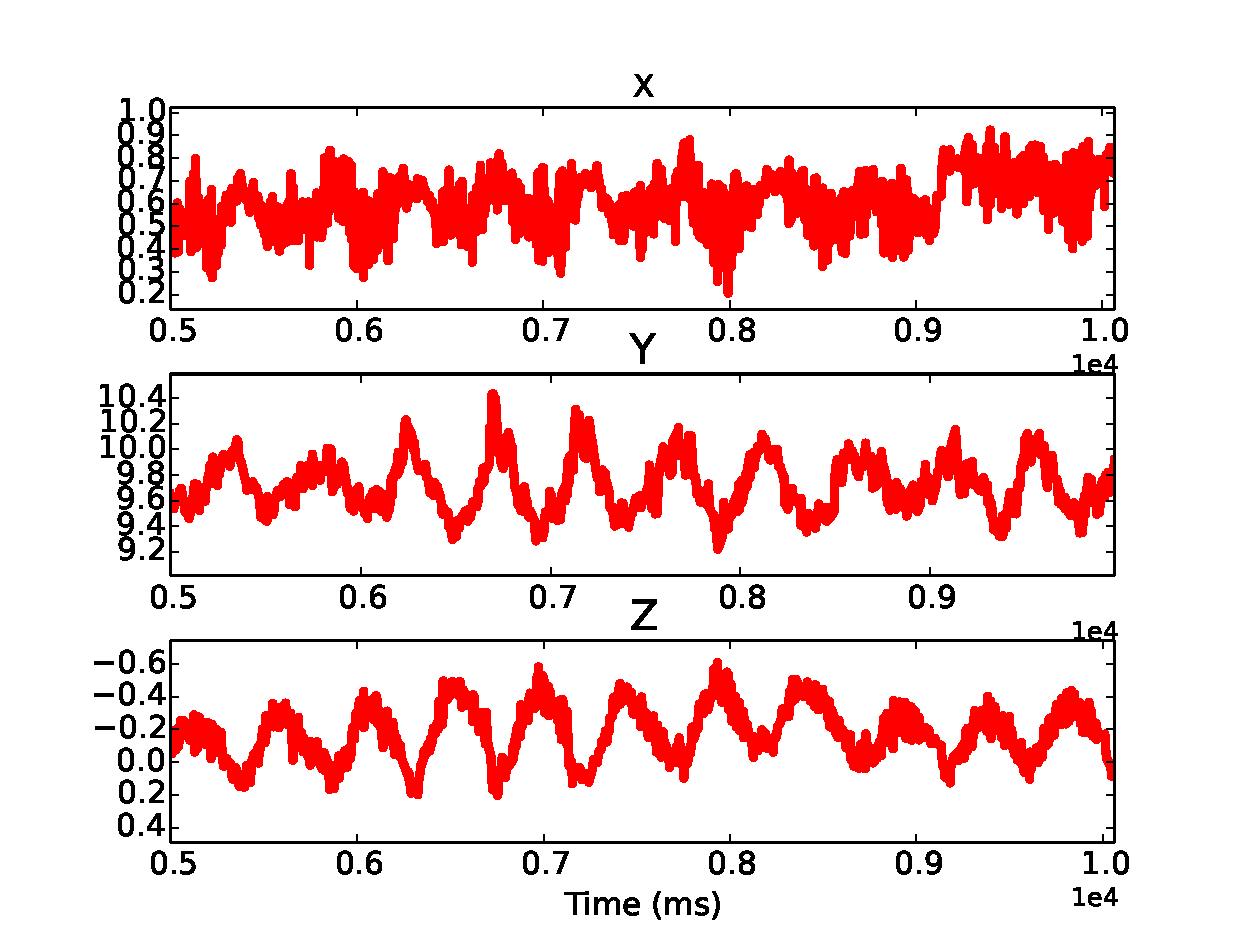
\includegraphics [width=.33\linewidth]{../mobisys_paper/fig/raw_sub3.eps}\\
(a) User 1& (b) User 2 & (c) User 3 \\
\end{tabular}

\begin{tabular}{cc}
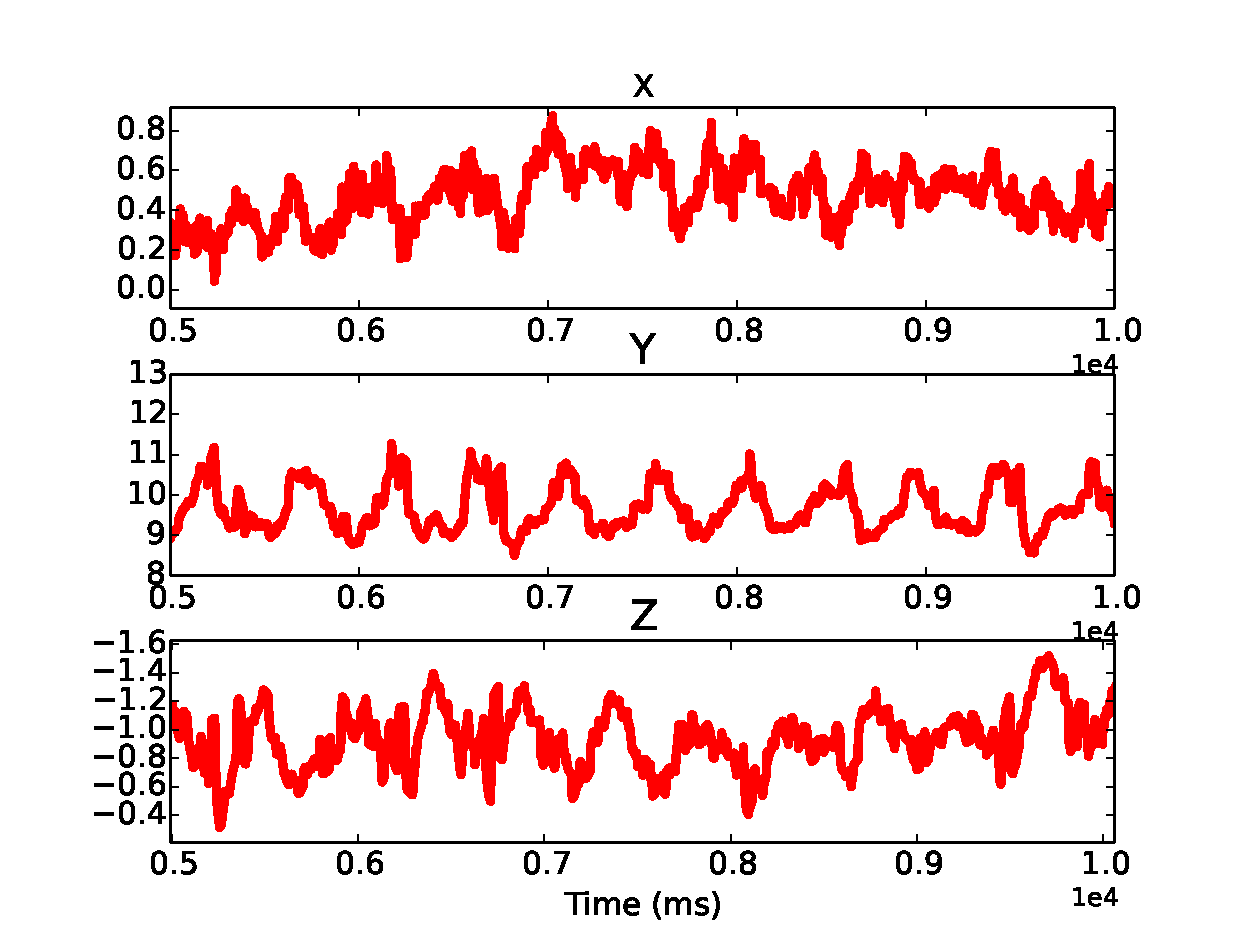
\includegraphics [width=.33\linewidth]{../mobisys_paper/fig/raw_sub4.eps}&
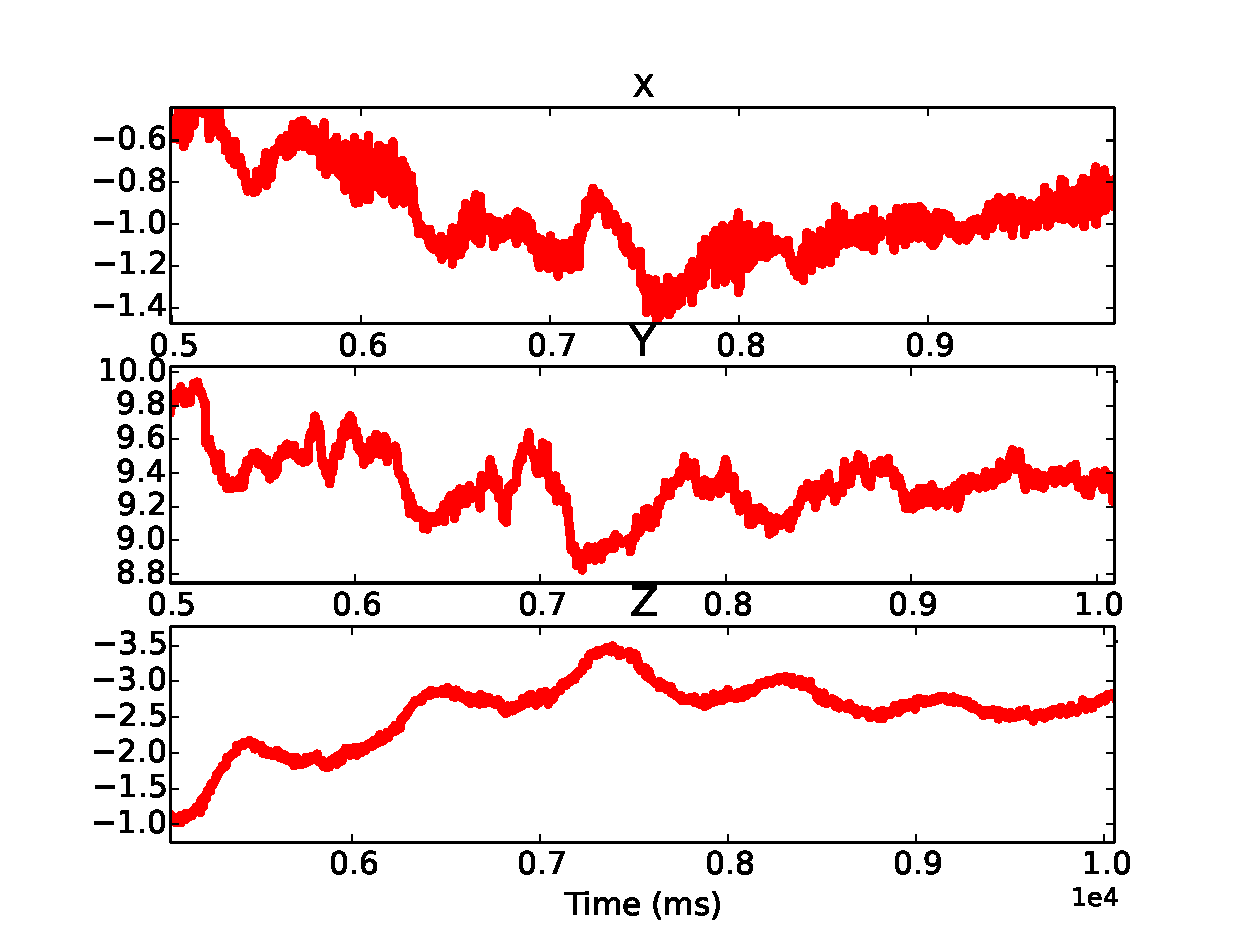
\includegraphics [width=.33\linewidth]{../mobisys_paper/fig/raw_sub5.eps}\\
(d) User 4& (e) User 5 \\
\end{tabular}
\end{center}
\caption{\label{fig:raw} These plots show the raw accelerometer data in the
time domain for five different users when they move their head in response to
a music track wearing the same Google glass. The plots
indicate that different users' head movement patterns appear distinctive from
each other. The five users wore a Google Glass (in turns) and listened to a
10 second audio snapshot of a pop song.}
\end{figure*}

\subsection{Background on Authenticating Wearable Devices}
Authentication mechanisms for a wearable device can broadly be divided into two
categories: (i) {\em Direct} authentication, where the users can directly
authenticate themselves to their wearable device using the input/output
interface and/or using signatures generated from the sensors available on the
device, and (ii) {\em Indirect} authentication, where a secondary device --
typically the user's smartphone -- is used as a medium for authentication.
Today's commercially available wearable devices predominantly use the latter
approach where users login to their wearable devices through their smartphone
-- using a PIN or an email account.
%A select few gadgets, for example the Google Glass or fitbit, require the
%users to register their device to their user specific accounts (gmail for
%Google Glass), which can also be perceived as an indirect mechanism for
%authentication.


Unlike the indirect approaches, that require a wearable device is registered to
and connected (wireless) to a smartphone, direct
mechanisms can leverage the built-in interfaces and sensors on the
wearable device. The fact that wearable devices relate significantly to ``what we wear" on the
human body, biometrics can play a key role for direct authentication to wearable
devices. Biometrics allow a system to identify a user based upon ``who you
are" (i.e., her physiology) instead of ``what you
have'' (i.e., ID cards) or `` what you remember'' (i.e.,
passwords)~\cite{jain2004introduction,o2003comparing,yampolskiy2007motor}.
Physiological biometrics such as DNA, ear shape, face, fingerprint,
hand/finger geometry,
iris, odor, palm-print, retinal scan, and voice, have been very effective and
widely used in many prototype and commercial authentication systems.
In addition, body shape such as body height, width, and body-part proportions
can also be used as biometric cues to identify different
people~\cite{collins2002silhouette}. Even ``soft'' characteristics such as
body weight and fat percentage have been considered as secondary biometrics
for authentication purposes~\cite{ailisto2006soft}. However, biometrics are
not prominently used in wearable devices commercially available today, though
there have been specific point commercial designs (e.g., Nymi~\cite{nymi}). This can be attributed to the
fact that biometrics would require the specific hardware/sensor available on
the wearable device. Also the overheads for physiological biometrics in
wearable devices can be high, in both, cost for hardware as well as
integration and computing.

An other approach to direct authentication is using behavioral biometrics
where unique signatures from human behavior (subconscious
or in response to external stimulus) provide cues for differentiating and
authenticating users. For example, it has been shown that gait (e.g.,
stride length, the
amount of arm swing) when the user is walking or
running is a reliable identification cue, and irrespective of the
environment~\cite{stevenage1999visual}. Okumura et.al.~\cite{okumura2006study}
have shown that the human arm swing patterns can be used to create signatures
to authenticate to their cell-phones. Monrose
et.al.~\cite{monrose2000keystroke} show that keystroke rhythms, when
users type on the keyboard, that include typing dynamics such as how
long is a keystroke, how far is between consecutive strokes, and how is the
pressure exerted on each key, can be used as a biometric to authenticate
users. Similarly, mouse usage dynamics~\cite{jorgensen2011mouse} and touchpad
touching dynamics~\cite{bo2013silentsense,de2012touch} have also been shown to
serve as potential biometrics.

In comparison to other means of authentication, behavioral biometric
authentication can offer a more convenient (than physiological biometrics),
and more secure (than indirect authentication) solution for wearable device
authentication. With the increasing off-the-shelf
availability and (almost) unlimited access to the sensors on the wearables, it
has become possible to generate and/or infer unique behavioral signatures
specific to users. We use these rationale as a motivation for our proposed
design of a behavioral biometric based authentication that generates unique
signatures from user's body movements.
We design an authentication system, dubbed {\em Headbanger}, for wearable
devices by monitoring user's unique body-movement patterns (e.g., head movements, arm movements, and hand movements) in response to an
external audio stimulus.

%\vspace{4pt}{\bf Head-movements as a behavioral biometric.}

\subsection{Body Movement as a Behavioral Biometric}
\label{subsec:headmovements}

%As such, authenticating a user involves comparing her sensor
%readings with the pre-recorded glass owner's sensor readings.
%Our design assumes that there is only one owner per glass, and we can easily
%extend our scheme to handle the cases with multiple owners.
%Figure~\ref{fig:sysarch} presents the system architecture of the \systemname,
%and in the following section, we will discuss each component of this design
%in more detail.

According to~\cite{jain2004introduction}, a human characteristic can be
considered as biometric as long as it is \emph{universal}, \emph{distinctive},
\emph{repeatable}, and \emph{collectible}. With the advancements in
wearable computer designs it is becoming easier for collecting body movement
patterns using the built-in sensors (e.g., accelerometer sensor, gyroscope sensor, motion sensor, etc). Such sensors are
available on most wearable devices available today, thus
making body movements that are universally available {\em collectible} in all
aspects. It has been shown~\cite{zentner2010rhythmic} that most people move
their body as a natural response to external rhythmic stimuli such as music --
even at a very early age, infants respond to music and their movements speed
up with the increasing rhythm speed. We observed that even adults naturally
perform head movements or hand movements when listening to a fast beat audio track.

Based on a
preliminary analysis of the accelerometer signals from five Google Glass
users, we also observed (see Figure~\ref{fig:raw} (a)-(e)) that these users
{\em repeatedly} showed unique and {\em distinctive} head-movement patterns,
when listening to the same music beats on the head-worn device.
Motivated by this observation we hypothesize that head movements
can be a good behavioral biometric characteristic to authenticate
users to their smart glass.
%We next formally present the design of our system that
%utilizes head-movement patterns as behavioral biometric signature

\vspace{4pt}\textbf{Example Body Movement Patterns:} Depending upon specific wearable devices, we can focus on different body parts. For example, head-mounted devices such as smart glasses/goggles can easily capture a user's head movements; wrist-mounted devices such as smart watches can easily capture a user's arm/hand movements; ***SL: finger-mounted device such as smart rings can easily capture a user's finger/palm movements; foot-mounted devices such as smart running shoes can easily capture user's gait. *** To facilitate natural and repeatable body movements, we can play short, fast-tempo music tracks on the wearable devices, and then measure the movement using built-in sensors such as accelerometer, gyroscope and pressure sensor. In addition, eye lid movements such as blinking or winking can also be easily captured by head-mounted devices; for example, Google glass is  with infrared proximity sensor to detect blinking and winking.

***YZ: Sugang, any other body movements we can study? ***
%to authenticate smart glass users.

\begin{figure}
\centering
\includegraphics[width=.5\columnwidth]{../mobisys_paper/fig/headbanger-illustrate.png}
\caption{Illustration of Headbanger. The head-worn device authenticates the
right user based on signatures generated from head-movement patterns in
response to an audio snapshot played on the device.}
\label{fig:illustrate}
\end{figure}



\subsection{Overview of ~\systemname}
We envision that our proposed system will be used as an authentication interface on the wearable device.  The system will run as a service in the device upon power-up, similar to the screen-lock in smartphones or the head-nod interface on Google
Glass~\cite{googleglass}. Upon usage, a short duration audio track
will be played on the device, and the user makes body movements in
response to the audio. ~\systemname will then go through the following steps:
\begin{itemize}
\item {\em Sensor data collection}: ~\systemname~records the body movements
in the form of raw sensor signals (e.g., accelerometer or gyroscope) using the built-in
sensors on the wearable device.

\item {\em Filtering}: The raw sensor signals are then filtered by applying filters such as low-pass filter to remove records of extraneous motion.

\item {\em Signature generation}: The filtered signals are then
processed to obtain the unique features for each user-audio pair.


\item {\em Classification}: The signatures are classified
to different users based on data mining and machine learning strategies, and
labeled to the corresponding user.

\item {\em Authentication}: The head-movement signature generated
during system operation is compared with the original user-audio pair
signature, and the user is authenticated access if there is a plausible match.
\end{itemize}

The illustration of~\systemname~is shown in Figure~\ref{fig:illustrate}.




\subsection{Research Challenges}
Specifically, the proposed research effort consists of the following thrusts:
\begin{itemize}
\item Developing signal processing and learning algorithms that can accurately identifying each user's body movement patterns.

\item Developing a light-weight, low-cost authentication system that can run on wearable devices efficiently.

\end{itemize}
